
\documentclass[tikz,convert={outfile=\jobname.svg},20pt]{standalone}
\newcommand{\sla}{s}
\newcommand{\pos}[1]{\mathtt{x}_{#1}}
\newcommand{\si}[1]{s_{#1}}
\newcommand{\Bo}{\mathcal{B}}
\newcommand{\nor}{n}
\begin{document}

%\centering
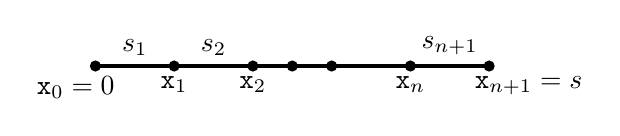
\begin{tikzpicture}[line width = 1.1pt]
 \draw (0,0) -- (5,0);
 
 \draw (-0.25,0) node[anchor=north] {${ \pos{0}=0}$};
%  \draw (0,0) node[anchor=south] {$0$};
  \draw [fill=black](0,0) circle (.05cm);
 
  %\draw (5,0) node[anchor=south] {$s$};
  \draw (5.5,0) node[anchor=north] {$\pos{n+1}=\sla$};    
   \draw [fill=black] (5,0) circle (.05cm);
   
     \draw (.5,0) node[anchor=south] {$\si{1}$};
  \draw (1.0,0) node[anchor=north] {$\pos{1}$};    
    \draw [fill=black](1.0,0) circle (.05cm);
   
     \draw (1.5,0) node[anchor=south] {$\si{2}$};
  \draw (2.0,0) node[anchor=north] {$\pos{2}$};    
    \draw [fill=black] (2.0,0) circle (.05cm);
   
    \draw  (2.5,0) circle (.05cm);
 \draw  (3.0,0) circle (.05cm);
   
   
   \draw (4.5,0) node[anchor=south] {$\si{n+1}$};
  \draw (4.0,0) node[anchor=north] {$\pos{n}$};    
 \draw [fill=black] (4.0,0) circle (.05cm);
   
\end{tikzpicture}
\end{document}
